%! Author = Андрей
%! Date = 05.11.2022

%----------------------------------------------------------------------------------------
%	TITLE AND CONTACT INFORMATION
%----------------------------------------------------------------------------------------

	\begin{minipage}{0.1\textwidth}
		\begin{figure}[H]
			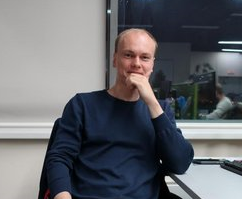
\includegraphics[width=3.5cm]{1}
		\end{figure}
	\end{minipage}
	\hfill
    \begin{minipage}[t]{0.35\textwidth} % 45% of the page width for name
        %\vspace{-\baselineskip} % Required for vertically aligning minipages

        % If your name is very short, use just one of the lines below
        % If your name is very long, reduce the font size or make the minipage wider and reduce the others proportionately
        \colorbox{black}{{\HUGE\textcolor{white}{\textbf{\MakeUppercase{Andrei}}}}} % First name

        \colorbox{black}{{\HUGE\textcolor{white}{\textbf{\MakeUppercase{Briukhov}}}}} % Last name

        \vspace{6pt}

        {\huge Java/Kotlin developer} % Career or current job title
    \end{minipage}
    \begin{minipage}[t]{0.25\textwidth} % 27.5% of the page width for the first row of icons
        %\vspace{-\baselineskip} % Required for vertically aligning minipages

        % The first parameter is the FontAwesome icon name, the second is the box size and the third is the text
        % Other icons can be found by referring to fontawesome.pdf (supplied with the template) and using the word after \fa in the command for the icon you want
        %\icon{MapMarker}{12}{}\\

        \icon{Globe}{12}{Brazil, São Paulo}\\
        \icon{Calendar}{12}{25-05-1986, 36 yo}\\
        \icon{Phone}{12}{+55 (11) 97791-8776}\\
        \icon{At}{12}{\href{mailto:andreybr611@gmail.com}{andreybr611@gmail.com}}

    \end{minipage}
    \begin{minipage}[t]{0.2\textwidth} % 27.5% of the page width for the second row of icons
        %\vspace{-\baselineskip} % Required for vertically aligning minipages

        % The first parameter is the FontAwesome icon name, the second is the box size and the third is the text
        % Other icons can be found by referring to fontawesome.pdf (supplied with the template) and using the word after \fa in the command for the icon you want
        \icon{Linkedin}{12}{\href{https://www.linkedin.com/in/tbw777}{tbw777}} \\
        \icon{Skype}{12}{\href{https://join.skype.com/invite/mjNUCTfkejKc}{Click to chat}} \\
        \icon{Twitter}{12}{\href{https://twitter.com/ABriukhov}{ABriukhov}} \\
        \icon{Whatsapp}{12}{\href{https://wa.me/5511977918776}{Click to chat}}\\
%        \icon{MessageText}{12}{Generated in \LaTeX}
    \end{minipage}



    \vspace{0.4cm}

%----------------------------------------------------------------------------------------
%	INTRODUCTION, SKILLS AND TECHNOLOGIES
%----------------------------------------------------------------------------------------

    \begin{minipage}[t]{0.76\textwidth} % 40% of the page width for the introduction text
        \vspace{-\baselineskip} % Required for vertically aligning minipages
        
        \cvsect{Why me?}

        \begin{itemize}[leftmargin=.0in]
        	\setlength\itemsep{0em}
            \item I understand the structure of systems, possible schemes for building interactions and frequent mistakes
            \item I develop safe and reliable systems with highest quality of code maintability and extensability
            \item I prefer versatility, consistency, always looking for systemic scalable automated solutions
            \item I adhere to the principles: \textbf{SDLC}, \textbf{SOLID}, \textbf{KISS}, \textbf{DRY}, \textbf{YAGNI}
            \item Typical architecture and design patterns in implementation priority
            \item I choose approaches and prioritize based on context and requirements
            \item My overall experience is about \underline{17} years of commercial development (since 2005)
            \item Successful experience in solving business-critical project tasks from the first job
        \end{itemize}

    \end{minipage}
    \hfill % Whitespace between
    \begin{minipage}[t]{0.20\textwidth} % 50% of the page for the skills bar chart
        \vspace{-\baselineskip}
        
        \cvsect{My stack}
        
        \icon{Java}{10}{\textbf{Java}} \& \textbf{Kotlin} plus:
        \begin{itemize}[leftmargin=.2in]
        	\setlength\itemsep{0em}
        	\item Assembler
        	\item Camunda
        	\item C/C++
           	\item Groovy
           	\item JavaScript
           	\item Shell script
            
            %\item{JavaScript: Node.js, JQuery, React, Angular}
            %\item{C/C++ (C89/C99/C++2003/Other)}
            %\item{Assembler x86: real mode, unreal mode, protected mode, MSRs}
            
            \item \LaTeX
        \end{itemize}
    \end{minipage}

\vspace{0.4cm}